\documentclass[journal,12pt,twocolumn]{IEEEtran}
\usepackage{romannum}
\usepackage{float}
\usepackage{setspace}
\usepackage{gensymb}
\singlespacing
\usepackage[cmex10]{amsmath}
\usepackage{amsthm}
\usepackage{mathrsfs}
\usepackage{txfonts}
\usepackage{stfloats}
\usepackage{bm}
\usepackage{cite}
\usepackage{cases}
\usepackage{subfig}
\usepackage{longtable}
\usepackage{multirow}
\usepackage{enumitem}
\usepackage{mathtools}
\usepackage{steinmetz}
\usepackage{tikz}
\usepackage{circuitikz}
\usepackage{verbatim}
\usepackage{tfrupee}
\usepackage[breaklinks=true]{hyperref}
\usepackage{tkz-euclide}
\usetikzlibrary{calc,math}
\usepackage{listings}
    \usepackage{color}                                            %%
    \usepackage{array}                                            %%
    \usepackage{longtable}                                        %%
    \usepackage{calc}                                             %%
    \usepackage{multirow}                                         %%
    \usepackage{hhline}                                           %%
    \usepackage{ifthen}                                           %%
  %optionally (for landscape tables embedded in another document): %%
    \usepackage{lscape}     
\usepackage{multicol}
\usepackage{chngcntr}
\DeclareMathOperator*{\Res}{Res}
\renewcommand\thesection{\arabic{section}}
\renewcommand\thesubsection{\thesection.\arabic{subsection}}
\renewcommand\thesubsubsection{\thesubsection.\arabic{subsubsection}}

\renewcommand\thesectiondis{\arabic{section}}
\renewcommand\thesubsectiondis{\thesectiondis.\arabic{subsection}}
\renewcommand\thesubsubsectiondis{\thesubsectiondis.\arabic{subsubsection}}

% correct bad hyphenation here
\hyphenation{op-tical net-works semi-conduc-tor}
\def\inputGnumericTable{}                                 %%

\lstset{
frame=single, 
breaklines=true,
columns=fullflexible
}

\begin{document}


\newtheorem{theorem}{Theorem}[section]
\newtheorem{problem}{Problem}
\newtheorem{proposition}{Proposition}[section]
\newtheorem{lemma}{Lemma}[section]
\newtheorem{corollary}[theorem]{Corollary}
\newtheorem{example}{Example}[section]
\newtheorem{definition}[problem]{Definition}
\newcommand{\BEQA}{\begin{eqnarray}}
\newcommand{\EEQA}{\end{eqnarray}}
\newcommand{\define}{\stackrel{\triangle}{=}}

\bibliographystyle{IEEEtran}
\providecommand{\mbf}{\mathbf}
\providecommand{\pr}[1]{\ensuremath{\Pr\left(#1\right)}}
\providecommand{\qfunc}[1]{\ensuremath{Q\left(#1\right)}}
\providecommand{\sbrak}[1]{\ensuremath{{}\left[#1\right]}}
\providecommand{\lsbrak}[1]{\ensuremath{{}\left[#1\right.}}
\providecommand{\rsbrak}[1]{\ensuremath{{}\left.#1\right]}}
\providecommand{\brak}[1]{\ensuremath{\left(#1\right)}}
\providecommand{\lbrak}[1]{\ensuremath{\left(#1\right.}}
\providecommand{\rbrak}[1]{\ensuremath{\left.#1\right)}}
\providecommand{\cbrak}[1]{\ensuremath{\left\{#1\right\}}}
\providecommand{\lcbrak}[1]{\ensuremath{\left\{#1\right.}}
\providecommand{\rcbrak}[1]{\ensuremath{\left.#1\right\}}}
\theoremstyle{remark}
\newtheorem{rem}{Remark}
\newcommand{\sgn}{\mathop{\mathrm{sgn}}}
\providecommand{\abs}[1]{\left\vert#1\right\vert}
\providecommand{\res}[1]{\Res\displaylimits_{#1}} 
\providecommand{\norm}[1]{\left\lVert#1\right\rVert}
\providecommand{\mtx}[1]{\mathbf{#1}}
\providecommand{\mean}[1]{E\left[ #1 \right]}
\providecommand{\fourier}{\overset{\mathcal{F}}{ \rightleftharpoons}}
\providecommand{\system}{\overset{\mathcal{H}}{ \longleftrightarrow}}
\newcommand{\solution}{\noindent \textbf{Solution: }}
\newcommand{\cosec}{\,\text{cosec}\,}
\providecommand{\dec}[2]{\ensuremath{\overset{#1}{\underset{#2}{\gtrless}}}}
\newcommand{\myvec}[1]{\ensuremath{\begin{pmatrix}#1\end{pmatrix}}}
\newcommand{\mydet}[1]{\ensuremath{\begin{vmatrix}#1\end{vmatrix}}}
\numberwithin{equation}{subsection}
\makeatletter
\@addtoreset{figure}{problem}
\makeatother

\let\StandardTheFigure\thefigure
\let\vec\mathbf
\renewcommand{\thefigure}{\theproblem}



\def\putbox#1#2#3{\makebox[0in][l]{\makebox[#1][l]{}\raisebox{\baselineskip}[0in][0in]{\raisebox{#2}[0in][0in]{#3}}}}
     \def\rightbox#1{\makebox[0in][r]{#1}}
     \def\centbox#1{\makebox[0in]{#1}}
     \def\topbox#1{\raisebox{-\baselineskip}[0in][0in]{#1}}
     \def\midbox#1{\raisebox{-0.5\baselineskip}[0in][0in]{#1}}

\vspace{3cm}


\title{Assignment 1}
\author{Jaswanth Chowdary Madala}





% make the title area
\maketitle

\newpage

%\tableofcontents

\bigskip

\renewcommand{\thefigure}{\theenumi}
\renewcommand{\thetable}{\theenumi}

\begin{enumerate}
\item Find the shortest distance between the lines $l_1$ and $l_2$ whose vector equations are ${\overrightarrow{r} = \hat{i}+\hat{j}+\lambda(2\hat{i}-\hat{j}+\hat{k})}$ and ${\overrightarrow{r} = 2\hat{i}+\hat{j}-\hat{k}+\mu(3\hat{i}-5\hat{j}+2\hat{k})}$

\textbf{Solution:} The lines $l_1$ and $l_2$ in vector form can be written as
\begin{align}
\vec{x} &= \myvec{1\\1\\0} + \lambda_1\myvec{2\\-1\\1}\\
\vec{x} &= \myvec{2\\1\\-1} + \lambda_2\myvec{3\\-5\\2}\\
\vec{x_1} = \myvec{1\\1\\0},\, \vec{x_2} &= \myvec{2\\1\\-1}, \,\vec{m_1} = \myvec{2\\-1\\1}, \, \vec{m_2} = \myvec{3\\-5\\2}
\end{align}
The distance between the lines is given by,
\begin{align}
d &= \norm{\brak{\vec{x_2}+ \lambda_2\vec{m_2}} - \brak{\vec{x_1}+ \lambda_1\vec{m_1}}}\\
\implies d &= \norm{\vec{x_2}-\vec{x_1}-\lambda_1\vec{m_1}+\lambda_2\vec{m_2}} \label{eq:1}
\end{align}
Consider the following definitions
\begin{align}
\vec{A} &\triangleq \vec{x_2} - \vec{x_1} \label{eq:2}\\
\vec{M} &\triangleq \myvec{\vec{m_1} & \vec{m_2}} \label{eq:3}\\
\bm{\lambda} &\triangleq \myvec{\lambda_1\\-\lambda_2} \label{eq:4}
\end{align}
From the above definitions \eqref{eq:2}, \eqref{eq:3}, \eqref{eq:4} we get,
\begin{align}
d = \norm{\vec{A}-\vec{M}\bm{\lambda}}
\end{align}
Here we have the values of $\vec{A}, \vec{M}$ as
\begin{align}
\vec{M} &= \myvec{2&3\\-1&-5\\1&2}\\
\vec{A} &= \myvec{1\\0\\-1}
\end{align}
Consider the function
\begin{align}
f\brak{\bm{\lambda}} = \norm{\vec{A}-\vec{M}\bm{\lambda}}^2
\end{align}
The given problem can be formulated as 
\begin{align}
\min_{\bm{\lambda}} f\brak{\bm{\lambda}} &= \bm{\lambda}^{\top}\vec{M}^\top\vec{M}\bm{\lambda} - 2\vec{A}^\top\vec{M}\bm{\lambda}+\norm{\vec{A}}^2 \label{eq:5}
\end{align}
Here we have,
\begin{align}
\vec{M}^\top\vec{M} &= \myvec{6&13 \\ 13&38}\\
\vec{A}^\top\vec{M} &= \myvec{1&1}\\
\norm{\vec{A}}^2 &= 2
\end{align}
A numerical solution for \eqref{eq:5} is obtained as
\begin{align}
\bm{\lambda}_{n+1}&=\bm{\lambda}_{n}-\alpha \nabla f\brak{\bm{\lambda_n}} \label{eq:6}
\end{align}
where $\lambda_0$ is an inital guess and $\alpha$ is a variable parameter. These parameters decide how fast the algorithm converges. Here the gradient is given by,
\begin{align}
\nabla f\brak{\bm{\lambda}} = 2\vec{M}^\top\vec{M} \bm{\lambda} - 2\brak{\vec{A}^\top\vec{M}}^\top
\end{align}

From \eqref{eq:6} we get
\begin{align}
\bm{\lambda}_{n+1} &= \bm{\lambda}_{n} -\alpha \brak{2\vec{M}^\top\vec{M} \bm{\lambda}_n - 2\vec{M}^\top\vec{A}}
\end{align}
By taking the parameters as listed in the below table
\begin{table}[h]
\centering
%%%%%%%%%%%%%%%%%%%%%%%%%%%%%%%%%%%%%%%%%%%%%%%%%%%%%%%%%%%%%%%%%%%%%%
%%                                                                  %%
%%  This is a LaTeX2e table fragment exported from Gnumeric.        %%
%%                                                                  %%
%%%%%%%%%%%%%%%%%%%%%%%%%%%%%%%%%%%%%%%%%%%%%%%%%%%%%%%%%%%%%%%%%%%%%%

\begin{center}
\begin{tabular}{|c|c|c|}
\hline
\textbf{RV}& \textbf{Values} & \textbf{Description} \\ \hline
$X$		   & 	$\{0,1\}$	&  1st draw - 0: black card, 1: red card\\ \hline
$Y$ 		   & 	$\{0,1\}$	&  2nd draw - 0: black card, 1: red card\\ \hline
$X,Y$ 		   & 	$\{00\}$	&	2 cards drawn are black\\ \hline
\end{tabular}
\end{center}

\caption{}
\label{tab:1}
\end{table}

$\lambda$ obtained is
\begin{align}
\bm{\lambda} &= \myvec{0.4237 \\-0.1186}
\end{align}
The shortest distance is
\begin{align}
\min_{\bm{\lambda}} d &= 1.3019  
\end{align}

The shortest distance between the given lines is $1.3019$ units, and this answer matches with the other methods.

\begin{figure}[!ht]
\centering
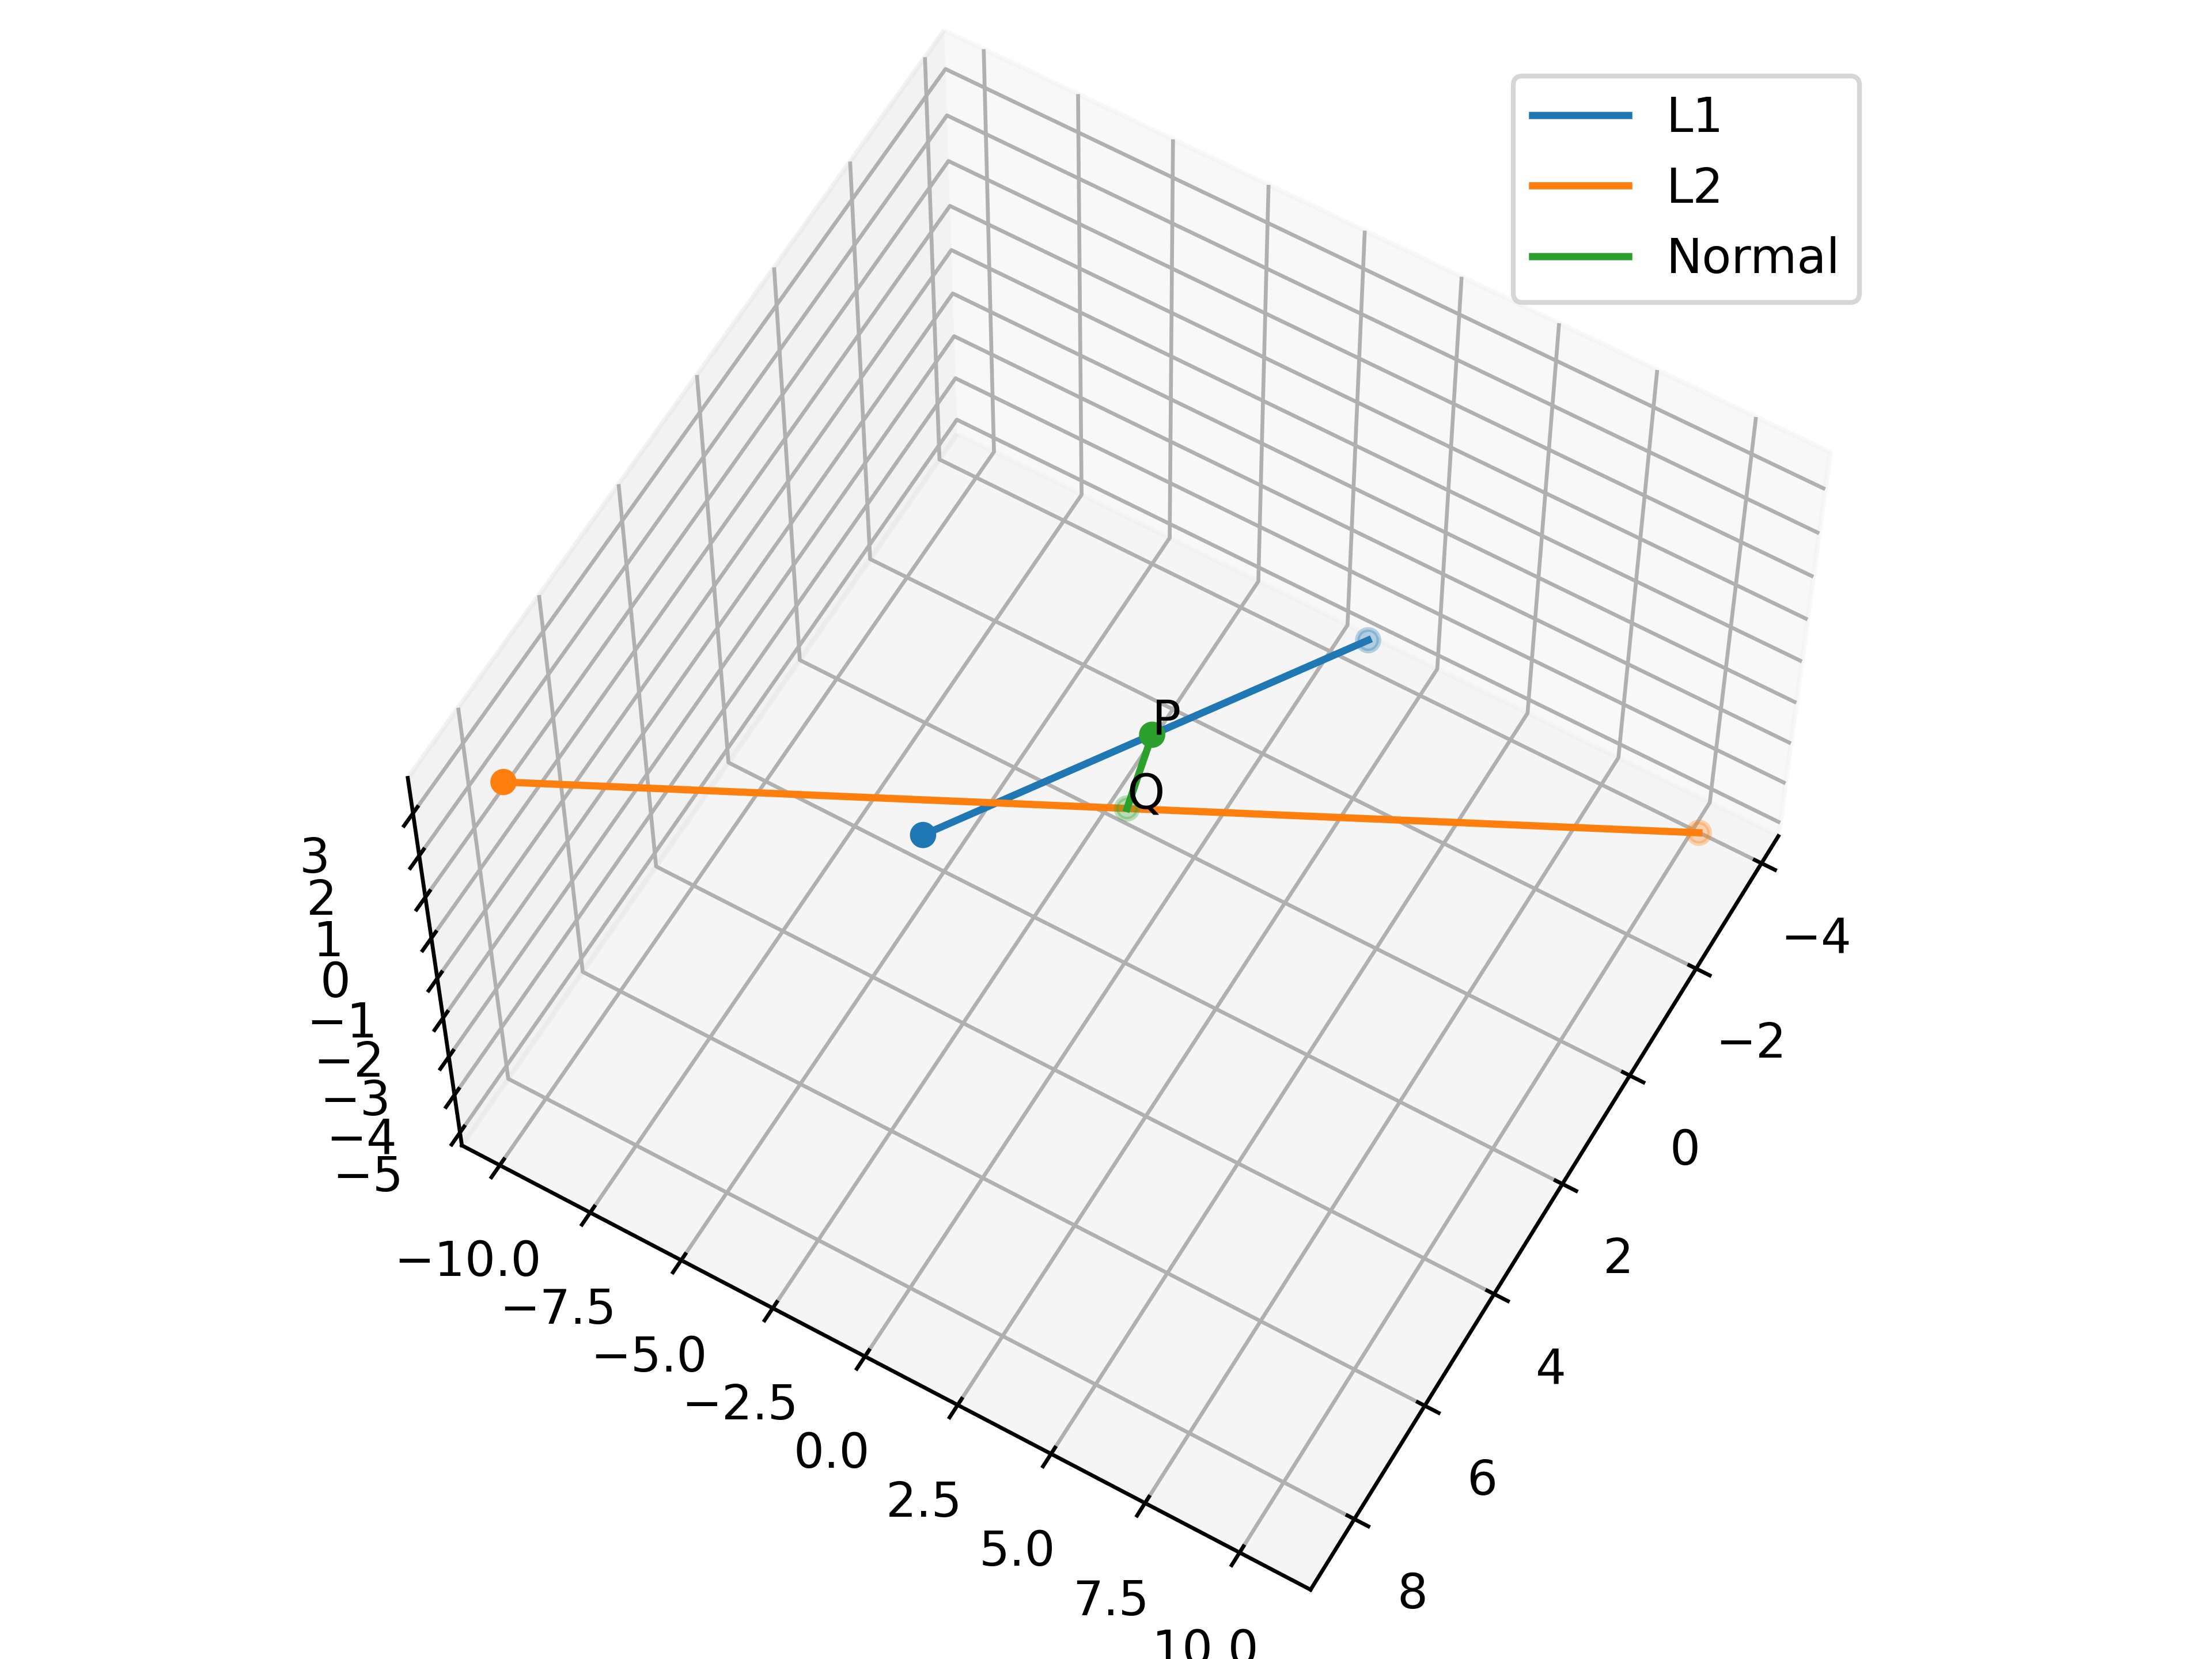
\includegraphics[width=\columnwidth]{./figs/skew.png}
\caption{$PQ$ is the required shortest distance.}
\end{figure}
\end{enumerate}
\end{document}